\documentclass[aspectratio=169]{beamer}

\usepackage[T1]{fontenc}
\usepackage[utf8]{inputenc}
\usepackage{lmodern}
\usepackage{xcolor}
\usepackage{tikz}
\usetikzlibrary{arrows.meta,positioning,fit,backgrounds,calc}
\usepackage{listings}
\usepackage{pifont}

%%─────────────────────────────────────────────────────────────────
%%  COLOURS — creamy off-white
%%─────────────────────────────────────────────────────────────────
\definecolor{creamBg}{HTML}{FAF6EE}
\definecolor{creamDk}{HTML}{EDE4CC}
\definecolor{creamMd}{HTML}{E4D8B8}
\definecolor{creamRl}{HTML}{C8B888}

\definecolor{inkK}{HTML}{1A1208}
\definecolor{inkB}{HTML}{2E1E08}
\definecolor{inkM}{HTML}{4A3418}

\definecolor{cTeal}{HTML}{1B5C5E}
\definecolor{lTeal}{HTML}{C6DEDE}
\definecolor{cAmber}{HTML}{9A5A10}
\definecolor{lAmber}{HTML}{F2DEB8}
\definecolor{cSage}{HTML}{3A6850}
\definecolor{lSage}{HTML}{C6DDD4}
\definecolor{cRust}{HTML}{8A2E18}
\definecolor{lRust}{HTML}{F0CFBF}
\definecolor{cInd}{HTML}{2E3480}
\definecolor{lInd}{HTML}{D0D2EE}
\definecolor{cOk}{HTML}{1A5E3A}
\definecolor{lOk}{HTML}{C4DDD0}

%%─────────────────────────────────────────────────────────────────
%%  BEAMER
%%─────────────────────────────────────────────────────────────────
\usetheme{default}
\usecolortheme{default}
\setbeamertemplate{navigation symbols}{}
\setbeamercolor{background canvas}{bg=creamBg}
\setbeamercolor{normal text}{fg=inkK}
\setbeamertemplate{itemize item}{\textcolor{cAmber}{\rule{5pt}{5pt}}}
\setbeamertemplate{itemize subitem}{\textcolor{cTeal}{\rule{4pt}{4pt}}}

\setbeamertemplate{frametitle}{%
  \vspace{9pt}%
  {\sffamily\Large\bfseries\color{inkB}\insertframetitle}%
  \ifx\insertframesubtitle\empty\else
    \\[2pt]{\sffamily\small\color{cTeal}\insertframesubtitle}%
  \fi
  \par\vspace{3pt}%
  {\color{creamRl}\hrule height 1pt}%
  \vspace{3pt}%
}

\setbeamertemplate{footline}{%
  \begin{beamercolorbox}[wd=\paperwidth,ht=16pt,dp=5pt]{}%
    \hspace{14pt}%
    {\tiny\color{inkM}\sffamily Project Architecture \& Deployment}%
    \hfill
    {\tiny\color{inkM}\sffamily\insertframenumber/\inserttotalframenumber}%
    \hspace{14pt}%
  \end{beamercolorbox}%
}

%%─────────────────────────────────────────────────────────────────
%%  LISTINGS
%%─────────────────────────────────────────────────────────────────
\lstset{
  backgroundcolor=\color{creamDk},
  basicstyle=\ttfamily\scriptsize\color{inkB},
  keywordstyle=\bfseries\color{cTeal},
  commentstyle=\itshape\color{cSage},
  stringstyle=\color{cAmber},
  breaklines=true,
  frame=l, framerule=2pt, rulecolor=\color{cAmber},
  xleftmargin=8pt, tabsize=2, showstringspaces=false,
  aboveskip=3pt, belowskip=3pt,
}

%%─────────────────────────────────────────────────────────────────
%%  TIKZ STYLES  — ALL flat, no parameterised keys
%%─────────────────────────────────────────────────────────────────
\tikzset{
  %% ── named service boxes ─────────────────────────────────────
  NTeal/.style={draw=cTeal, fill=lTeal, rounded corners=5pt,
    minimum width=2.8cm, minimum height=1.2cm,
    align=center, font=\sffamily\small\bfseries, text=cTeal,
    inner sep=5pt},
  NAmber/.style={draw=cAmber, fill=lAmber, rounded corners=5pt,
    minimum width=2.8cm, minimum height=1.2cm,
    align=center, font=\sffamily\small\bfseries, text=cAmber,
    inner sep=5pt},
  NSage/.style={draw=cSage, fill=lSage, rounded corners=5pt,
    minimum width=2.8cm, minimum height=1.2cm,
    align=center, font=\sffamily\small\bfseries, text=cSage,
    inner sep=5pt},
  NRust/.style={draw=cRust, fill=lRust, rounded corners=5pt,
    minimum width=2.8cm, minimum height=1.2cm,
    align=center, font=\sffamily\small\bfseries, text=cRust,
    inner sep=5pt},
  NInd/.style={draw=cInd, fill=lInd, rounded corners=5pt,
    minimum width=2.8cm, minimum height=1.2cm,
    align=center, font=\sffamily\small\bfseries, text=cInd,
    inner sep=5pt},
  NGray/.style={draw=creamRl, fill=creamDk, rounded corners=5pt,
    minimum width=2.8cm, minimum height=1.2cm,
    align=center, font=\sffamily\small\bfseries, text=inkM,
    inner sep=5pt},
  %% ── flow boxes ───────────────────────────────────────────────
  Flow/.style={draw=creamRl, fill=creamDk, rounded corners=4pt,
    minimum width=11cm, minimum height=0.75cm,
    align=center, font=\sffamily\small, text=inkK, inner sep=5pt},
  Trig/.style={draw=cAmber, fill=lAmber, rounded corners=5pt,
    minimum width=11cm, minimum height=0.80cm,
    align=center, font=\sffamily\small\bfseries, text=inkB,
    inner sep=5pt},
  Good/.style={draw=cOk, fill=lOk, rounded corners=4pt,
    minimum width=11cm, minimum height=0.75cm,
    align=center, font=\sffamily\small\bfseries, text=cOk,
    inner sep=5pt},
  PhTeal/.style={draw=cTeal, fill=lTeal, rounded corners=4pt,
    minimum width=11cm, minimum height=0.75cm,
    align=center, font=\sffamily\small, text=inkK, inner sep=5pt},
  PhSage/.style={draw=cSage, fill=lSage, rounded corners=4pt,
    minimum width=11cm, minimum height=0.75cm,
    align=center, font=\sffamily\small, text=inkK, inner sep=5pt},
  PhRust/.style={draw=cRust, fill=lRust, rounded corners=4pt,
    minimum width=11cm, minimum height=0.75cm,
    align=center, font=\sffamily\small, text=inkK, inner sep=5pt},
  PhAmber/.style={draw=cAmber, fill=lAmber, rounded corners=4pt,
    minimum width=11cm, minimum height=0.75cm,
    align=center, font=\sffamily\small, text=inkK, inner sep=5pt},
  %% ── wide flow boxes (CI/CD slide) ───────────────────────────
  WFlow/.style={draw=creamRl, fill=creamDk, rounded corners=4pt,
    minimum width=12cm, minimum height=0.72cm,
    align=center, font=\sffamily\small, text=inkK, inner sep=5pt},
  WTrig/.style={draw=cAmber, fill=lAmber, rounded corners=5pt,
    minimum width=12cm, minimum height=0.78cm,
    align=center, font=\sffamily\small\bfseries, text=inkB,
    inner sep=5pt},
  WGood/.style={draw=cOk, fill=lOk, rounded corners=4pt,
    minimum width=12cm, minimum height=0.72cm,
    align=center, font=\sffamily\small\bfseries, text=cOk,
    inner sep=5pt},
  WTeal/.style={draw=cTeal, fill=lTeal, rounded corners=4pt,
    minimum width=12cm, minimum height=0.68cm,
    align=center, font=\sffamily\small\bfseries, text=cTeal,
    inner sep=5pt},
  WAmberH/.style={draw=cAmber, fill=lAmber, rounded corners=4pt,
    minimum width=12cm, minimum height=0.68cm,
    align=center, font=\sffamily\small\bfseries, text=cAmber,
    inner sep=5pt},
  %% ── narrow flow (request flow) ───────────────────────────────
  NFlow/.style={draw=creamRl, fill=creamDk, rounded corners=4pt,
    minimum width=6.4cm, minimum height=0.68cm,
    align=center, font=\sffamily\tiny, text=inkK, inner sep=4pt},
  NTrig/.style={draw=cAmber, fill=lAmber, rounded corners=4pt,
    minimum width=6.4cm, minimum height=0.72cm,
    align=center, font=\sffamily\tiny\bfseries, text=inkB,
    inner sep=4pt},
  NGood/.style={draw=cOk, fill=lOk, rounded corners=4pt,
    minimum width=6.4cm, minimum height=0.68cm,
    align=center, font=\sffamily\tiny\bfseries, text=cOk,
    inner sep=4pt},
  %% ── summary cards ────────────────────────────────────────────
  CAmber/.style={draw=cAmber, fill=lAmber, rounded corners=4pt,
    minimum width=6.6cm, minimum height=0.75cm,
    align=left, inner xsep=7pt, font=\sffamily\small, text=inkK},
  CTeal/.style={draw=cTeal, fill=lTeal, rounded corners=4pt,
    minimum width=6.6cm, minimum height=0.75cm,
    align=left, inner xsep=7pt, font=\sffamily\small, text=inkK},
  CSage/.style={draw=cSage, fill=lSage, rounded corners=4pt,
    minimum width=6.6cm, minimum height=0.75cm,
    align=left, inner xsep=7pt, font=\sffamily\small, text=inkK},
  CRust/.style={draw=cRust, fill=lRust, rounded corners=4pt,
    minimum width=6.6cm, minimum height=0.75cm,
    align=left, inner xsep=7pt, font=\sffamily\small, text=inkK},
  CInd/.style={draw=cInd, fill=lInd, rounded corners=4pt,
    minimum width=6.6cm, minimum height=0.75cm,
    align=left, inner xsep=7pt, font=\sffamily\small, text=inkK},
  %% ── arrows ───────────────────────────────────────────────────
  AR/.style={-{Stealth[length=7pt,width=5pt]},
             line width=1.8pt, color=cAmber},
  AT/.style={-{Stealth[length=6pt,width=4pt]},
             line width=1.4pt, color=cTeal},
  AD/.style={-{Stealth[length=5pt]}, dashed,
             line width=0.8pt, color=inkM},
}

%%─────────────────────────────────────────────────────────────────
%%  HELPERS
%%─────────────────────────────────────────────────────────────────
\newcommand{\CM}{\textcolor{cOk}{\ding{51}}\ }

%% Pill tag — safe, no # inside tikz node style
\newcommand{\pill}[2]{%
  \begin{tikzpicture}[baseline=-2pt]
    \node[draw=#1, fill=#1!15, rounded corners=3pt,
          inner xsep=5pt, inner ysep=2pt,
          font=\sffamily\tiny\bfseries, text=#1]{#2};
  \end{tikzpicture}%
}

%% Coloured vertical rule bullet
\newcommand{\VR}[1]{\textcolor{#1}{\rule{3pt}{9pt}}\ }

%%═════════════════════════════════════════════════════════════════
\begin{document}
%%═════════════════════════════════════════════════════════════════

%%─────────────────────────────────────────────────────────────────
%%  SLIDE 1 — TITLE
%%─────────────────────────────────────────────────────────────────
{%
\setbeamertemplate{footline}{}
\begin{frame}
\begin{tikzpicture}[remember picture,overlay]
  \fill[cAmber]
    (current page.north west)
    rectangle ([xshift=0.7cm]current page.south west);
  \fill[lAmber]
    ([xshift=0.7cm]current page.north west)
    rectangle ([xshift=0.85cm]current page.south west);
  \fill[creamDk]
    (current page.north west)
    rectangle ([yshift=-1.8cm]current page.north east);
  \fill[creamRl]
    ([yshift=-1.8cm]current page.north west)
    rectangle ([yshift=-1.92cm]current page.north east);
  \fill[creamDk]
    (current page.south west)
    rectangle ([yshift=1.2cm]current page.south east);
  \fill[creamRl]
    ([yshift=1.2cm]current page.south west)
    rectangle ([yshift=1.08cm]current page.south east);
  \foreach \R in {0.5,1.0,1.5,2.0,2.5}{
    \draw[creamRl,line width=0.5pt]
      (current page.north east) ++(-\R cm,0) arc(90:180:\R cm);
  }
\end{tikzpicture}

\vspace{0.5cm}
\hspace{0.9cm}%
\begin{minipage}{0.88\textwidth}
  {\sffamily\tiny\color{cTeal}\MakeUppercase{Technical Presentation}}

  \vspace{0.35cm}
  {\sffamily\fontsize{30}{36}\selectfont\bfseries\color{inkB}
    Project Architecture}\\[4pt]
  {\sffamily\fontsize{17}{22}\selectfont\color{cTeal}
    \& Automated Deployment Flow}

  \vspace{0.35cm}
  {\color{creamRl}\rule{9cm}{1.2pt}}
  \vspace{0.3cm}

  {\small\color{inkM}
    High-level walkthrough of the mono-repo stack,\\
    service architecture, and CI/CD pipeline.}

  \vspace{0.5cm}
  \pill{cTeal}{Node.js}\
  \pill{cAmber}{React}\
  \pill{cSage}{PostgreSQL}\
  \pill{cRust}{Docker}\
  \pill{cInd}{GitHub Actions}\
  \pill{cTeal}{Nginx}\
  \pill{cAmber}{OCI}

  \vspace{0.6cm}
  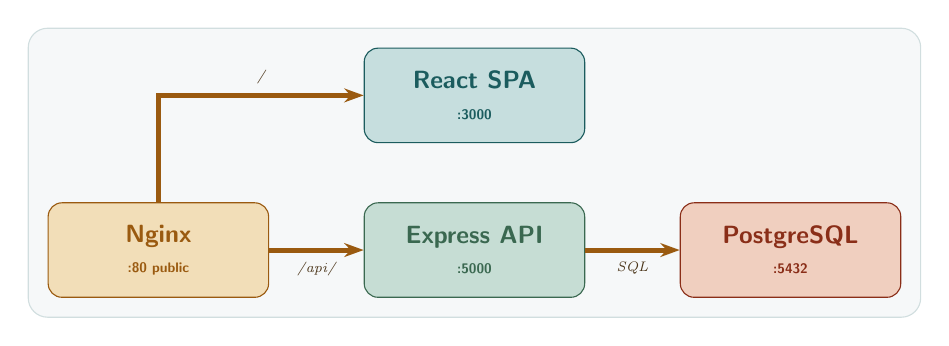
\begin{tikzpicture}[node distance=0.85cm and 1.2cm]
    \node[NAmber] (ng) {\textbf{Nginx}\\\tiny :80 public};
    \node[NSage, right=1.2cm of ng] (be)
      {\textbf{Express API}\\\tiny :5000};
    \node[NTeal, above=0.75cm of be] (fe)
      {\textbf{React SPA}\\\tiny :3000};
    \node[NRust, right=1.2cm of be] (db)
      {\textbf{PostgreSQL}\\\tiny :5432};
    \draw[AR] (ng) -- (be)
      node[midway,below,font=\tiny\itshape,text=inkM]{/api/};
    \draw[AR] (ng.north) |- (fe.west)
      node[near end,above,font=\tiny\itshape,text=inkM]{/};
    \draw[AR] (be) -- (db)
      node[midway,below,font=\tiny\itshape,text=inkM]{SQL};
    \begin{scope}[on background layer]
      \node[draw=cTeal!20,fill=cTeal!4,rounded corners=7pt,
            fit=(fe)(be)(db)(ng),inner sep=7pt]{};
    \end{scope}
  \end{tikzpicture}
\end{minipage}
\end{frame}
}

%%─────────────────────────────────────────────────────────────────
%%  SLIDE 2 — WHAT IS THIS PROJECT?
%%─────────────────────────────────────────────────────────────────
\begin{frame}{What Is This Project?}
\vspace{0.1cm}
\begin{columns}[T]

\column{0.52\textwidth}
\begin{tikzpicture}
  \node[draw=creamRl, fill=creamDk, rounded corners=7pt,
        minimum width=7.5cm, minimum height=5.6cm,
        inner sep=12pt, align=left] (card) {};
  \node[anchor=north west, text width=6.8cm]
    at ([xshift=3pt,yshift=-3pt]card.north west) {
    \vspace{2pt}
    {\sffamily\bfseries\color{inkB} A full-stack containerised web app}
    \vspace{5pt}

    \begin{itemize}[leftmargin=1.2em, itemsep=4pt]
      \item \textbf{Backend} \textemdash\ Node.js + Express REST API
      \item \textbf{Frontend} \textemdash\ React SPA built with Vite
      \item \textbf{Database} \textemdash\ PostgreSQL, persistent storage
      \item \textbf{Proxy} \textemdash\ Nginx, single public entry-point
      \item \textbf{Packaging} \textemdash\ Docker containers throughout
      \item \textbf{Delivery} \textemdash\ CI/CD via GitHub Actions
    \end{itemize}

    \vspace{7pt}
    {\small\color{inkM}
      All four services live in one \textbf{mono-repo},\\
      wired by a single \texttt{docker-compose.yml}.}
  };
\end{tikzpicture}

\column{0.46\textwidth}
\vspace{0.2cm}
{\sffamily\small\bfseries\color{cTeal} Guiding principles}
\vspace{5pt}


\begin{tikzpicture}
  \node[CAmber]
    {\VR{cAmber}\textbf{One command} \textemdash\ just \texttt{git push}};
\end{tikzpicture}
\vspace{3pt}

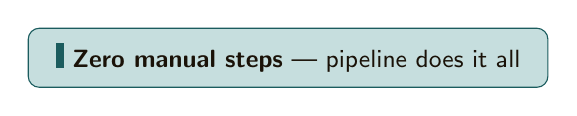
\begin{tikzpicture}
  \node[CTeal]
    {\VR{cTeal}\textbf{Zero manual steps} \textemdash\ pipeline does it all};
\end{tikzpicture}
\vspace{3pt}


\begin{tikzpicture}
  \node[CSage]
    {\VR{cSage}\textbf{Data safe} \textemdash\ pgdata volume persists};
\end{tikzpicture}
\vspace{3pt}

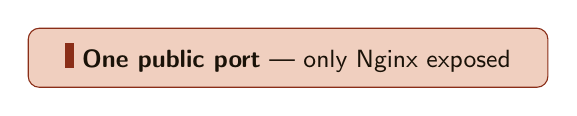
\begin{tikzpicture}
  \node[CRust]
    {\VR{cRust}\textbf{One public port} \textemdash\ only Nginx exposed};
\end{tikzpicture}

\end{columns}
\end{frame}

%%─────────────────────────────────────────────────────────────────
%%  SLIDE 3 — SERVICE ARCHITECTURE
%%─────────────────────────────────────────────────────────────────
\begin{frame}{Service Architecture}
\framesubtitle{Four services \textemdash\ one Docker network \textemdash\ one public port}
\vspace{0.05cm}
\centering
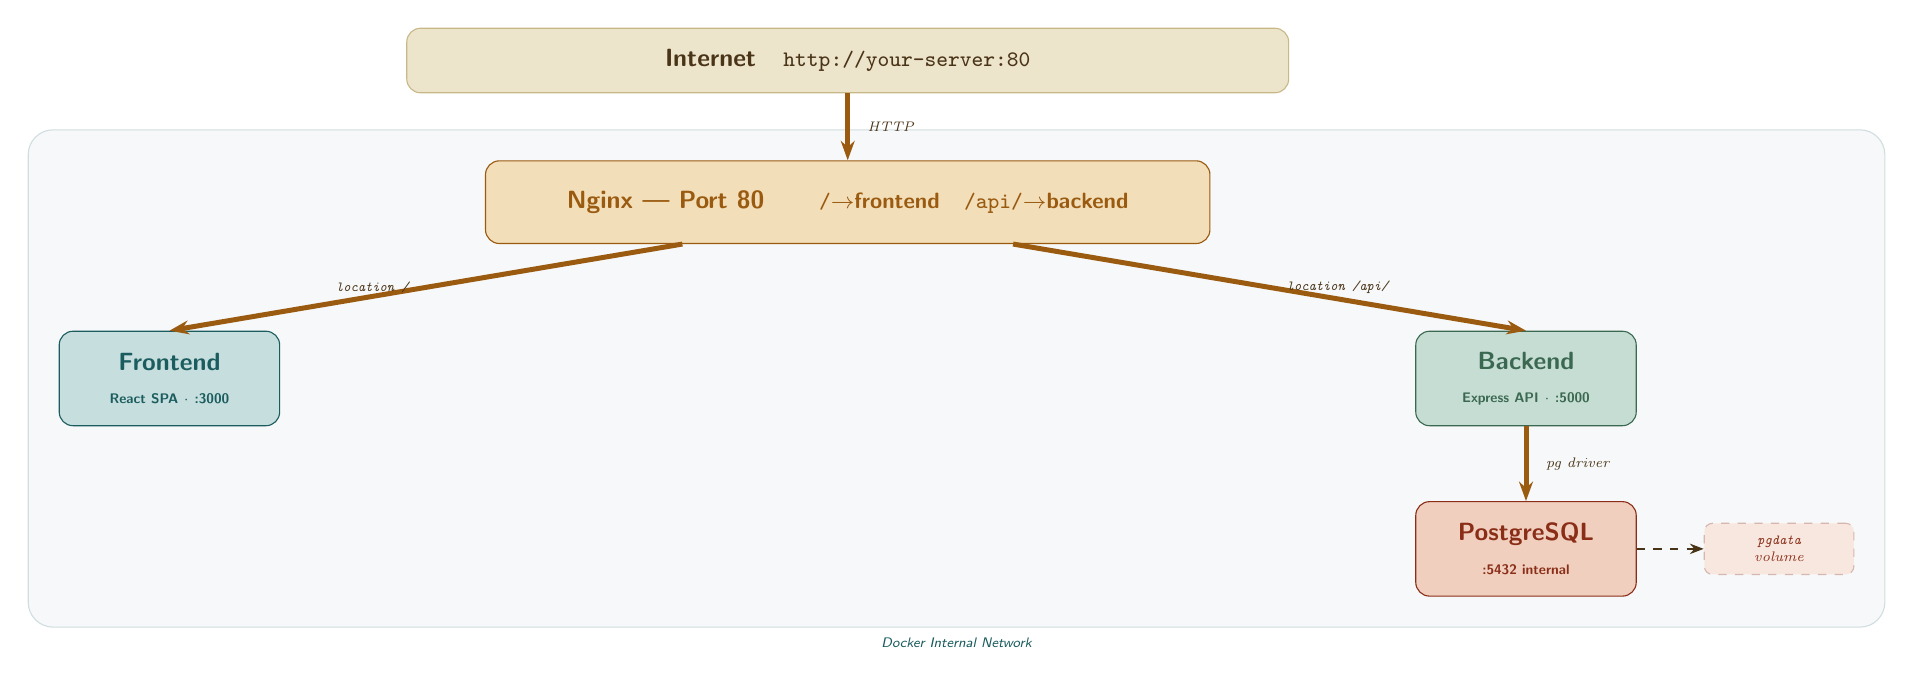
\begin{tikzpicture}[node distance=0.9cm and 1.9cm,
                    every node/.style={font=\small}]

  \node[NGray, minimum width=11.2cm, minimum height=0.82cm] (net) at (0,0)
    {{\sffamily\bfseries\color{inkM} Internet}\quad
     \footnotesize\texttt{http://your-server:80}};

  \node[NAmber, minimum width=9.2cm, minimum height=1.05cm,
        below=0.85cm of net] (nginx)
    {\textbf{Nginx \textemdash\ Port 80}\qquad
     \footnotesize\texttt{/}$\to$frontend\quad
     \texttt{/api/}$\to$backend};

  \node[NTeal, below left=1.1cm and 2.6cm of nginx] (fe)
    {\textbf{Frontend}\\[1pt]\tiny React SPA $\cdot$ :3000};

  \node[NSage, below right=1.1cm and 2.6cm of nginx] (be)
    {\textbf{Backend}\\[1pt]\tiny Express API $\cdot$ :5000};

  \node[NRust, below=0.95cm of be] (pg)
    {\textbf{PostgreSQL}\\[1pt]\tiny :5432 internal};

  \node[draw=cRust!35, fill=lRust!50, rounded corners=3pt, dashed,
        minimum width=1.9cm, minimum height=0.65cm,
        align=center, font=\tiny\itshape, text=cRust,
        right=0.85cm of pg] (vol)
    {\texttt{pgdata}\\volume};

  \draw[AR] (net) -- (nginx)
    node[midway,right=3pt,font=\tiny\itshape,text=inkM]{HTTP};
  \draw[AR] ([xshift=-2.1cm]nginx.south) -- (fe.north)
    node[midway,left=2pt,font=\tiny\itshape,text=inkM]
    {\texttt{location /}};
  \draw[AR] ([xshift=2.1cm]nginx.south) -- (be.north)
    node[midway,right=2pt,font=\tiny\itshape,text=inkM]
    {\texttt{location /api/}};
  \draw[AR] (be) -- (pg)
    node[midway,right=3pt,font=\tiny\itshape,text=inkM]{pg driver};
  \draw[AD] (pg.east) -- (vol.west);

  \begin{scope}[on background layer]
    \node[draw=cTeal!20, fill=cTeal!4, rounded corners=9pt,
          fit=(fe)(be)(pg)(vol)(nginx), inner sep=11pt,
          label={[font=\tiny\sffamily\itshape,
                  text=cTeal]below:Docker Internal Network}]
    {};
  \end{scope}
\end{tikzpicture}
\end{frame}

%%─────────────────────────────────────────────────────────────────
%%  SLIDE 4 — TECH STACK
%%─────────────────────────────────────────────────────────────────
\begin{frame}{Tech Stack at a Glance}
\vspace{0.2cm}
\begin{columns}[T]

\column{0.24\textwidth}
\begin{tikzpicture}
  \node[draw=cTeal, fill=lTeal, rounded corners=6pt,
        minimum width=3.5cm, inner sep=9pt, align=left] {
    {\sffamily\small\bfseries\color{cTeal} Backend}
    \vspace{3pt}

    {\tiny\color{inkB}
      \textbf{Node.js} 22 Alpine\\[2pt]
      \textbf{Express} 5.x\\[2pt]
      \textbf{pg} driver 8.x\\[2pt]
      node-pg-migrate\\[2pt]
      dotenv $\cdot$ cors}
  };
\end{tikzpicture}

\column{0.24\textwidth}
\begin{tikzpicture}
  \node[draw=cAmber, fill=lAmber, rounded corners=6pt,
        minimum width=3.5cm, inner sep=9pt, align=left] {
    {\sffamily\small\bfseries\color{cAmber} Frontend}
    \vspace{3pt}

    {\tiny\color{inkB}
      \textbf{React} 18.x\\[2pt]
      \textbf{Vite} 5.x\\[2pt]
      \textbf{serve} 14.x\\[2pt]
      \phantom{x}\\[2pt]
      \phantom{x}}
  };
\end{tikzpicture}

\column{0.24\textwidth}
\begin{tikzpicture}
  \node[draw=cSage, fill=lSage, rounded corners=6pt,
        minimum width=3.5cm, inner sep=9pt, align=left] {
    {\sffamily\small\bfseries\color{cSage} Database}
    \vspace{3pt}

    {\tiny\color{inkB}
      \textbf{PostgreSQL} 16\\[2pt]
      Alpine image\\[2pt]
      Persistent volume\\[2pt]
      64 MB shared\_buf\\[2pt]
      max 50 connections}
  };
\end{tikzpicture}

\column{0.24\textwidth}
\begin{tikzpicture}
  \node[draw=cRust, fill=lRust, rounded corners=6pt,
        minimum width=3.5cm, inner sep=9pt, align=left] {
    {\sffamily\small\bfseries\color{cRust} DevOps}
    \vspace{3pt}

    {\tiny\color{inkB}
      \textbf{Docker} + Compose V2\\[2pt]
      \textbf{Nginx} Alpine\\[2pt]
      \textbf{GitHub Actions}\\[2pt]
      \textbf{OCIR} registry\\[2pt]
      OCI VM cloud}
  };
\end{tikzpicture}

\end{columns}

\vspace{0.4cm}
\centering
{\small\color{inkM}
  Alpine images keep sizes lean:
  Nginx $\approx$15 MB $\cdot$
  Frontend $\approx$150 MB $\cdot$
  Backend $\approx$180 MB}
\end{frame}

%%─────────────────────────────────────────────────────────────────
%%  SLIDE 5 — STARTUP SEQUENCE
%%─────────────────────────────────────────────────────────────────
\begin{frame}{Startup Sequence}
\framesubtitle{\texttt{docker compose up -d} \textemdash\ what happens next}
\vspace{0.1cm}
\centering
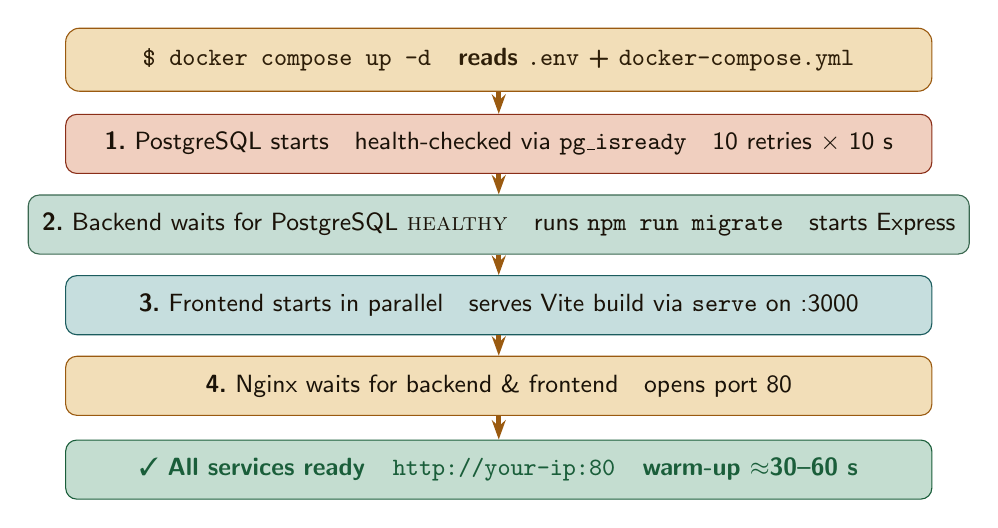
\begin{tikzpicture}[node distance=0.30cm, every node/.style={font=\small}]

  \node[Trig] (cmd)
    {\texttt{\$ docker compose up -d}\quad
     reads \texttt{.env} + \texttt{docker-compose.yml}};

  \node[PhRust, below=0.28cm of cmd] (pg)
    {\textbf{1.}\ PostgreSQL starts\quad
     health-checked via \texttt{pg\_isready}\quad
     10 retries $\times$ 10 s};

  \node[PhSage, below=0.26cm of pg] (be)
    {\textbf{2.}\ Backend waits for PostgreSQL \textsc{healthy}\quad
     runs \texttt{npm run migrate}\quad starts Express};

  \node[PhTeal, below=0.26cm of be] (fe)
    {\textbf{3.}\ Frontend starts in parallel\quad
     serves Vite build via \texttt{serve} on :3000};

  \node[PhAmber, below=0.26cm of fe] (ng)
    {\textbf{4.}\ Nginx waits for backend \& frontend\quad
     opens port 80};

  \node[Good, below=0.30cm of ng] (ok)
    {\CM All services ready\quad
     \texttt{http://your-ip:80}\quad
     warm-up $\approx$30--60 s};

  \draw[AR] (cmd) -- (pg);
  \draw[AR] (pg)  -- (be);
  \draw[AR] (be)  -- (fe);
  \draw[AR] (fe)  -- (ng);
  \draw[AR] (ng)  -- (ok);
\end{tikzpicture}
\end{frame}

%%─────────────────────────────────────────────────────────────────
%%  SLIDE 6 — DATABASE MIGRATIONS
%%─────────────────────────────────────────────────────────────────
\begin{frame}{Database Migrations}
\framesubtitle{Schema changes are automatic \textemdash\ no manual SQL}
\vspace{0.1cm}
\begin{columns}[T]

\column{0.47\textwidth}
{\sffamily\small\bfseries\color{cTeal} How it works}
\vspace{5pt}

\begin{itemize}[leftmargin=1.2em, itemsep=4pt]
  \item Files live in \texttt{backend/migrations/}
  \item On every start, \textbf{node-pg-migrate} runs
  \item Checks the \texttt{pgmigrations} table
  \item Only \emph{new} files applied \textemdash\ idempotent
  \item Express starts after migrate exits cleanly
\end{itemize}

\vspace{9pt}
{\sffamily\small\bfseries\color{cAmber} File naming}
\vspace{4pt}

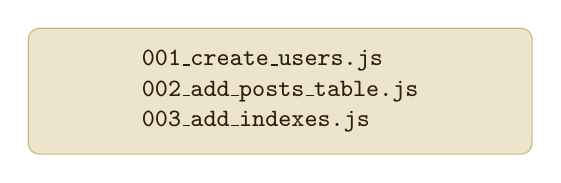
\begin{tikzpicture}
  \node[draw=creamRl, fill=creamDk, rounded corners=4pt,
        minimum width=6.4cm, inner sep=8pt,
        font=\ttfamily\small, text=inkB, align=left] {
    001\_create\_users.js\\
    002\_add\_posts\_table.js\\
    003\_add\_indexes.js
  };
\end{tikzpicture}

\column{0.51\textwidth}
{\sffamily\small\bfseries\color{cSage} Migration file}
\vspace{4pt}

\begin{lstlisting}
exports.up = pgm => {
  pgm.createTable('users', {
    id: {
      type: 'serial',
      primaryKey: true
    },
    name: {
      type: 'varchar(255)',
      notNull: true
    },
    email: {
      type: 'varchar(255)',
      unique: true
    },
  });
};

exports.down = pgm =>
  pgm.dropTable('users');
\end{lstlisting}

\vspace{4pt}
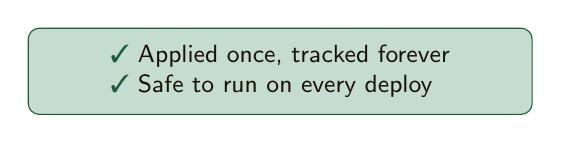
\begin{tikzpicture}
  \node[draw=cOk, fill=lOk, rounded corners=4pt,
        minimum width=6.4cm, inner sep=6pt,
        font=\sffamily\small, text=inkK, align=left] {
    \CM Applied once, tracked forever\\
    \CM Safe to run on every deploy
  };
\end{tikzpicture}

\end{columns}
\end{frame}

%%─────────────────────────────────────────────────────────────────
%%  SLIDE 7 — CI/CD PIPELINE
%%─────────────────────────────────────────────────────────────────
\begin{frame}{CI/CD Pipeline}
\framesubtitle{\texttt{git push main} $\to$ live in production \textemdash\ fully automated}
\vspace{0.05cm}
\centering
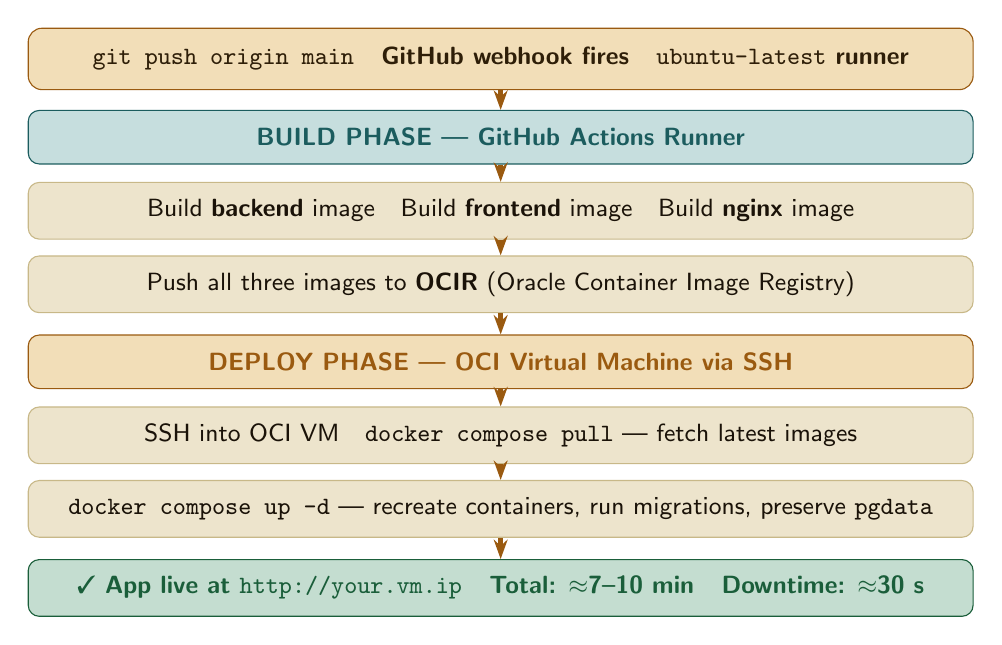
\begin{tikzpicture}[node distance=0.27cm, every node/.style={font=\small}]

  \node[WTrig] (push)
    {\texttt{git push origin main}\quad
     GitHub webhook fires\quad \texttt{ubuntu-latest} runner};

  \node[WTeal, below=0.25cm of push] (blbl)
    {BUILD PHASE \textemdash\ GitHub Actions Runner};

  \node[WFlow, below=0.22cm of blbl] (b1)
    {Build \textbf{backend} image\quad
     Build \textbf{frontend} image\quad
     Build \textbf{nginx} image};

  \node[WFlow, below=0.20cm of b1] (b2)
    {Push all three images to \textbf{OCIR}
     (Oracle Container Image Registry)};

  \node[WAmberH, below=0.27cm of b2] (dlbl)
    {DEPLOY PHASE \textemdash\ OCI Virtual Machine via SSH};

  \node[WFlow, below=0.22cm of dlbl] (d1)
    {SSH into OCI VM\quad
     \texttt{docker compose pull} \textemdash\ fetch latest images};

  \node[WFlow, below=0.20cm of d1] (d2)
    {\texttt{docker compose up -d} \textemdash\
     recreate containers, run migrations, preserve \texttt{pgdata}};

  \node[WGood, below=0.27cm of d2] (ok)
    {\CM App live at \texttt{http://your.vm.ip}\quad
     Total: $\approx$7--10 min\quad Downtime: $\approx$30 s};

  \draw[AR] (push) -- (blbl);
  \draw[AR] (blbl) -- (b1);
  \draw[AR] (b1)   -- (b2);
  \draw[AR] (b2)   -- (dlbl);
  \draw[AR] (dlbl) -- (d1);
  \draw[AR] (d1)   -- (d2);
  \draw[AR] (d2)   -- (ok);
\end{tikzpicture}
\end{frame}

%%─────────────────────────────────────────────────────────────────
%%  SLIDE 8 — SECRETS
%%─────────────────────────────────────────────────────────────────
\begin{frame}{Secrets \& Environment Variables}
\framesubtitle{Where credentials live and how they flow to containers}
\vspace{0.15cm}
\centering
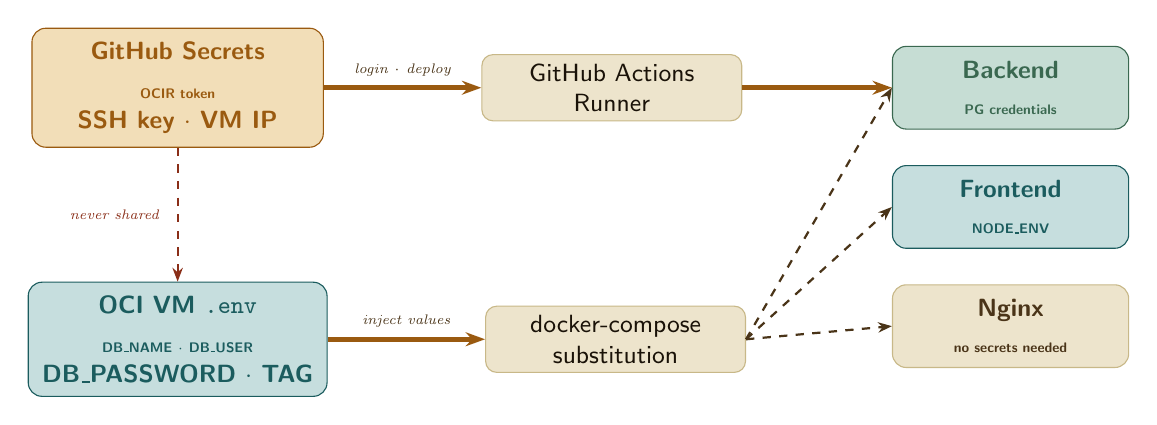
\begin{tikzpicture}[node distance=0.9cm and 2.2cm,
                    every node/.style={font=\small}]

  \node[NAmber, minimum width=3.7cm, minimum height=1.4cm] (gh)
    {\textbf{GitHub Secrets}\\[3pt]
     \tiny OCIR token\\SSH key $\cdot$ VM IP};

  \node[NTeal, minimum width=3.7cm, minimum height=1.4cm,
        below=1.7cm of gh] (env)
    {\textbf{OCI VM \texttt{.env}}\\[3pt]
     \tiny DB\_NAME $\cdot$ DB\_USER\\DB\_PASSWORD $\cdot$ TAG};

  \node[draw=creamRl, fill=creamDk, rounded corners=4pt,
        minimum width=3.3cm, minimum height=0.72cm,
        align=center, font=\sffamily\small, text=inkK,
        right=2.0cm of gh] (runner)
    {GitHub Actions\\Runner};

  \node[draw=creamRl, fill=creamDk, rounded corners=4pt,
        minimum width=3.3cm, minimum height=0.72cm,
        align=center, font=\sffamily\small, text=inkK,
        right=2.0cm of env] (dc)
    {docker-compose\\substitution};

  \node[NSage, minimum width=3.0cm, minimum height=1.05cm,
        right=1.9cm of runner] (be)
    {\textbf{Backend}\\[2pt]\tiny PG credentials};

  \node[NTeal, minimum width=3.0cm, minimum height=1.05cm,
        below=0.45cm of be] (fe)
    {\textbf{Frontend}\\[2pt]\tiny NODE\_ENV};

  \node[NGray, minimum width=3.0cm, minimum height=1.05cm,
        below=0.45cm of fe] (ng)
    {\textbf{Nginx}\\[2pt]\tiny no secrets needed};

  \draw[AR] (gh)  -- node[above,font=\tiny\itshape,text=inkM]
    {login $\cdot$ deploy} (runner);
  \draw[AR] (env) -- node[above,font=\tiny\itshape,text=inkM]
    {inject values} (dc);
  \draw[AR] (runner.east) -- (be.west);
  \draw[AD]  (dc.east) -- (be.west);
  \draw[AD]  (dc.east) -- (fe.west);
  \draw[AD]  (dc.east) -- (ng.west);
  \draw[AD,color=cRust] (gh.south) -- (env.north)
    node[midway,left=3pt,font=\tiny\itshape,text=cRust]{never shared};
\end{tikzpicture}
\end{frame}

%%─────────────────────────────────────────────────────────────────
%%  SLIDE 9 — NGINX ROUTING
%%─────────────────────────────────────────────────────────────────
\begin{frame}{Nginx Routing}
\framesubtitle{One port in \textemdash\ smart routing to the right service}
\vspace{0.1cm}
\begin{columns}[T]

\column{0.47\textwidth}
{\sffamily\small\bfseries\color{cAmber} Routing rules}
\vspace{5pt}


\begin{tikzpicture}
  \node[draw=cTeal, fill=lTeal, rounded corners=4pt,
        minimum width=6.4cm, minimum height=0.68cm,
        align=left, inner xsep=8pt,
        font=\ttfamily\small, text=inkK] {
    \textcolor{cTeal}{\textbf{/}}
    \hfill
    \textcolor{cTeal}{$\to$ Frontend :3000}
  };
\end{tikzpicture}
\vspace{3pt}


\begin{tikzpicture}
  \node[draw=cSage, fill=lSage, rounded corners=4pt,
        minimum width=6.4cm, minimum height=0.68cm,
        align=left, inner xsep=8pt,
        font=\ttfamily\small, text=inkK] {
    \textcolor{cSage}{\textbf{/api/}}
    \hfill
    \textcolor{cSage}{$\to$ Backend :5000}
  };
\end{tikzpicture}
\vspace{3pt}


\begin{tikzpicture}
  \node[draw=cSage, fill=lSage, rounded corners=4pt,
        minimum width=6.4cm, minimum height=0.68cm,
        align=left, inner xsep=8pt,
        font=\ttfamily\small, text=inkK] {
    \textcolor{cSage}{\textbf{/health}}
    \hfill
    \textcolor{cSage}{$\to$ Backend :5000}
  };
\end{tikzpicture}

\vspace{8pt}
{\sffamily\small\bfseries\color{cInd} Docker DNS}
\vspace{4pt}

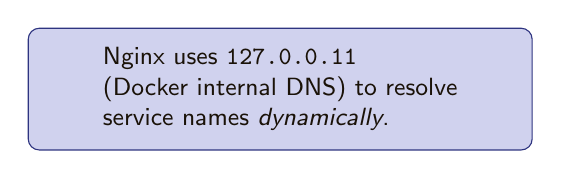
\begin{tikzpicture}
  \node[draw=cInd, fill=lInd, rounded corners=4pt,
        minimum width=6.4cm, inner sep=7pt,
        font=\sffamily\small, text=inkK, align=left] {
    Nginx uses \texttt{127.0.0.11}\\
    (Docker internal DNS) to resolve\\
    service names \emph{dynamically}.
  };
\end{tikzpicture}

\column{0.51\textwidth}
{\sffamily\small\bfseries\color{cSage} Request flow}
\vspace{5pt}

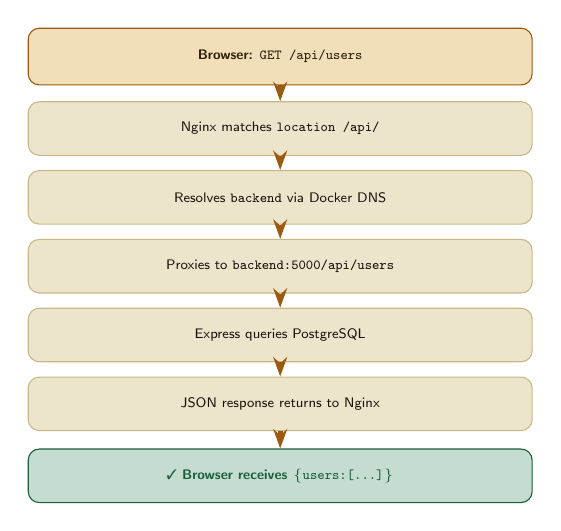
\begin{tikzpicture}[node distance=0.24cm]
  \node[NTrig] (u)  {Browser: \texttt{GET /api/users}};
  \node[NFlow, below=0.20cm of u]  (n1)
    {Nginx matches \texttt{location /api/}};
  \node[NFlow, below=0.18cm of n1] (n2)
    {Resolves \texttt{backend} via Docker DNS};
  \node[NFlow, below=0.18cm of n2] (n3)
    {Proxies to \texttt{backend:5000/api/users}};
  \node[NFlow, below=0.18cm of n3] (n4)
    {Express queries PostgreSQL};
  \node[NFlow, below=0.18cm of n4] (n5)
    {JSON response returns to Nginx};
  \node[NGood, below=0.22cm of n5] (ok)
    {\CM Browser receives \texttt{\{users:[...]\}}};

  \draw[AR] (u)  -- (n1);
  \draw[AR] (n1) -- (n2);
  \draw[AR] (n2) -- (n3);
  \draw[AR] (n3) -- (n4);
  \draw[AR] (n4) -- (n5);
  \draw[AR] (n5) -- (ok);
\end{tikzpicture}

\end{columns}
\end{frame}

%%─────────────────────────────────────────────────────────────────
%%  SLIDE 10 — SUMMARY
%%─────────────────────────────────────────────────────────────────
{%
\setbeamertemplate{footline}{}
\begin{frame}
\begin{tikzpicture}[remember picture,overlay]
  \fill[cAmber]
    (current page.north west)
    rectangle ([xshift=0.7cm]current page.south west);
  \fill[lAmber]
    ([xshift=0.7cm]current page.north west)
    rectangle ([xshift=0.85cm]current page.south west);
  \fill[creamDk]
    (current page.south west)
    rectangle ([yshift=1.3cm]current page.south east);
  \fill[creamRl]
    ([yshift=1.3cm]current page.south west)
    rectangle ([yshift=1.16cm]current page.south east);
\end{tikzpicture}

\vspace{0.3cm}
\hspace{0.8cm}%
\begin{minipage}{0.90\textwidth}

  {\sffamily\Large\bfseries\color{inkB} Summary}
  \par\vspace{2pt}
  {\color{creamRl}\hrule height 1pt}
  \vspace{0.4cm}

  \begin{columns}[T]

  \column{0.48\textwidth}

  
\begin{tikzpicture}
    \node[CAmber]
      {\textcolor{cAmber}{\ding{51}}\ \textbf{One command} \textemdash\ just \texttt{git push}};
  \end{tikzpicture}
  \vspace{3pt}

  
\begin{tikzpicture}
    \node[CTeal]
      {\textcolor{cTeal}{\ding{51}}\ \textbf{Auto migrations} \textemdash\ on every start};
  \end{tikzpicture}
  \vspace{3pt}

  
\begin{tikzpicture}
    \node[CSage]
      {\textcolor{cSage}{\ding{51}}\ \textbf{Data preserved} \textemdash\ pgdata persists};
  \end{tikzpicture}

  \column{0.48\textwidth}

  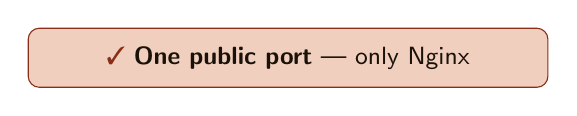
\begin{tikzpicture}
    \node[CRust]
      {\textcolor{cRust}{\ding{51}}\ \textbf{One public port} \textemdash\ only Nginx};
  \end{tikzpicture}
  \vspace{3pt}

  
\begin{tikzpicture}
    \node[CInd]
      {\textcolor{cInd}{\ding{51}}\ \textbf{Secrets safe} \textemdash\ never committed};
  \end{tikzpicture}
  \vspace{3pt}

  
\begin{tikzpicture}
    \node[CSage]
      {\textcolor{cSage}{\ding{51}}\ \textbf{Easy rollback} \textemdash\ revert or pin tag};
  \end{tikzpicture}

  \end{columns}

  \vspace{0.45cm}
  \centering
  {\color{creamRl}\rule{10cm}{0.8pt}}
  \vspace{0.25cm}

  {\small\color{inkM}
    \textbf{Stack:}
    Node.js $\cdot$ React $\cdot$ PostgreSQL $\cdot$
    Nginx $\cdot$ Docker $\cdot$ GitHub Actions $\cdot$ OCIR $\cdot$ OCI VM}

\end{minipage}
\end{frame}
}

\end{document}